%% LyX 2.0.5 created this file.  For more info, see http://www.lyx.org/.
%% Do not edit unless you really know what you are doing.
\documentclass[twocolumn]{article}
\usepackage[T1]{fontenc}
\usepackage[latin9]{inputenc}
\usepackage{geometry}
\geometry{verbose,tmargin=1in,bmargin=1in}
\usepackage{amsthm}
\usepackage{amsmath}
\usepackage{graphicx}

\makeatletter

%%%%%%%%%%%%%%%%%%%%%%%%%%%%%% LyX specific LaTeX commands.
%% Because html converters don't know tabularnewline
\providecommand{\tabularnewline}{\\}

%%%%%%%%%%%%%%%%%%%%%%%%%%%%%% Textclass specific LaTeX commands.
\numberwithin{equation}{section}
\numberwithin{figure}{section}

%%%%%%%%%%%%%%%%%%%%%%%%%%%%%% User specified LaTeX commands.
\usepackage{tikz}
\usetikzlibrary{arrows,fit,positioning}

\renewcommand*\theenumi{\alph{enumi}}
\renewcommand*\labelenumi{(\theenumi)}

\makeatletter
\def\imod#1{\allowbreak\mkern1mu({\operator@font mod}\,\,#1)}
\makeatother

\makeatother

\begin{document}

\title{User Review Rating Prediction}


\author{Sammy Leong, Ashish Bhatia}


\date{Dec 14, 2012}

\maketitle

\section*{Objective}

We're given a set of user review data each of which is associated
with a user rating. Our objective is to build a model that is able
to predict whether an unseen review is positive or negative.



\section*{Overview}

To solve this problem\cite{Qu:2010:BMR:1873781.1873884,li2010}, first
we evaluated a number of learning algorithms such as Logistic Regression,
Naive Bayes, and SVM on the original raw data as-is to get a sense
of their feasibility, capability, and speed. Then we developed our
own pre-processing pipeline to transform the original data to better
emphasize sentimental features, which we evaluated with one of the
learning algorithms. 

Based on our analysis, we removed several redundant and noisy features
to further improve the accuracy of our pipeline.

Project code (excluding Yelp data whose distribution is prohibited)
is available \href{https://github.com/ashishb/farsight}{https://github.com/ashishb/farsight}



\section*{Data Source}

\input{data_source.tex}


\section*{Success Metric}

Our goal is to find a learning algorithm along with data processing
techniques that give us the highest generalization accuracy. To do
this, we divided our data in half, trained with the first half, and
then tested with the second half. The former gives us the training
accuracy while the latter gives us the generalization accuracy.



\section*{First Attempt (Baseline)}

For our first attempt we focused on trying out various learning algorithms
on the original un-processed data as-is to get a sense of their capability
for our given problem. Another goal is to choose the fastest algorithm
which gives reasonably good results and use it to iterate while we
work on our pre-processing pipeline.


\subsection*{Results}

Here is a table that shows the training and generalization accuracies
for each learning algorithm, along with the time it took to run. The
experiments were done using $14000$ training examples and $14000$
testing examples.

\begin{center}
\begin{tabular}{|c|c|c|c|}
\hline 
 & Train & Test & Time\tabularnewline
\hline 
\multicolumn{4}{|c}{\emph{Matlab}}\tabularnewline
\hline 
Naive Bayes (mn) & $91.67$ & $81.27$ & $1.05$\tabularnewline
\hline 
\multicolumn{4}{|c}{\emph{Liblinear}}\tabularnewline
\hline 
Logistic Regression & $97.39$ & $81.67$ & $1.58$\tabularnewline
\hline 
L2-reg SVM (linear) & $99.69$ & $78.71$ & $2.86$\tabularnewline
\hline 
\multicolumn{4}{|c}{Libsvm}\tabularnewline
\hline 
C-SVM (linear) & $98.99$ & $78.86$ & $786$\tabularnewline
\hline 
C-SVM (radial) & $70.26$ & $69.68$ & $356$\tabularnewline
\hline 
C-SVM (sigmoid) & $65.11$ & $65.43$ & $359$\tabularnewline
\hline 
nu-SVM{*} (linear) & $87.78$ & $83.75$ & $277$\tabularnewline
\hline 
nu-SVM{*} (radial) & $88.80$ & $83.91$ & $296$\tabularnewline
\hline 
nu-SVM{*} (sigmoid) & $84.78$ & $81.49$ & $291$\tabularnewline
\hline 
\end{tabular}
\par\end{center}

{*} $nu=0.5$


\subsection*{Discussion}

Firstly, it's quite clear that liblinear runs significantly faster
than libsvm. For this reason, we will iterate using liblinear when
we evaluate the performance of various pre-processing techniques.
In particular, we will use logistic regression because it has higher
generalization accuracy than L2-regularized SVM with linear kernel.

Secondly, it appears that nu-SVM with $nu=0.5$ in this case improved
both the training and generalization accuracies significantly (as
compared to the counterpart C-SVM results). In fact, the we were able
to achieve the highest generalization accuracy using nu-SVM with the
radial basis kernel. The only issue is that it takes a very long time
to run. For this reason we will only revisit it after we've settled
on a good pre-processing pipeline.



\section*{Second Attempt}

For our second attempt, we focused on data processing and feature
selection with the goal of reducing the noise in the data as much
as possible. Here we only made use of logistic regression with $14000$
training examples and $14000$ testing examples. What follows are
the data processing techniques that we used.


\subsection*{Spell Correction}

The first thing we did was to apply spell checking on the reviews
and replace mispelled words with suggested corrections. The idea here
is that user reviews on the internet are often filled with misspelled
words. One positive review may contain the word ``good'' while another
may contain ``gooodi''. We want to treat both signals as representing
positive reviews.


\section*{Stemming}

After spell correction, we further consolidated words to their canonical
forms by applying stemming. For example, one positive review may contain
the word ``perfect'' while another may contain ``perfection''.
Again, we want to treat both signals as representing positive reviews.
Stemming converts both words to their root: ``perfect''.


\subsection*{Stopword Removal}

In this step we removed stop words that are believed to add little
relevence to reviews. Words like ``the'', ``I'', ``was'', etc.
are stop words and thus removed. One caveat is that we did not remove
the words ``no'' and ``not'' which will be explained in the bigram
generation section that follows.


\subsection*{Bi-gram Generation}

After spell correction, stemming, and stopword removal, we moved on
to bi-gram generation. This step is very important because it allows
us to capture semantics that are not captured in the uni-grams or
worst have opposite meaning altogether. For example ``really good''
is a much stronger signal for positive reviews than ``pretty good''
or just ``good''. Similarly, ``not good'', if captured inidividually
contains the word ``good'' which falsely indicates a positive review.
We can fix that by adding the bigram ``not-good'' but now we have
a problem where the review contains contradictory signals. To fix
that, we remove the word ``good'' and keep only ``not-good'' which
is a clear indication of a negative review.


\subsection*{Results}

Here is a table that shows the training and generalization accuracies.
The \emph{Individual} section shows experiment results where we used
each data processing technique individually. The \emph{Incremental}
section shows experiment results where we incrementally combined data
processing techniques. Finally, the \emph{Optimal} section shows experiment
results where we combined only data processing techniques that we
believe to give us optimal results.

\begin{center}
\begin{tabular}{|c|c|c|}
\hline 
 & Train & Test\tabularnewline
\hline 
\multicolumn{3}{|c}{\emph{Individual}}\tabularnewline
\hline 
\hline 
Baseline & $97.3931$ & $81.6759$\tabularnewline
\hline 
Spell Correction & $97.1862$ & $82.3517$\tabularnewline
\hline 
Stemming & $95.5655$ & $82.1586$\tabularnewline
\hline 
Stopword Rem & $97.1724$ & $82.6759$\tabularnewline
\hline 
Bi-grams & $99.9241$ & $84.4621$\tabularnewline
\hline 
\multicolumn{3}{|c|}{\emph{Incremental}}\tabularnewline
\hline 
\hline 
Baseline & $97.3931$ & $81.6759$\tabularnewline
\hline 
+ Spell Correction & $97.1862$ & $82.3517$\tabularnewline
\hline 
+ Stemming & $95.5034$ & $82.0000$\tabularnewline
\hline 
+ Stopword Rem & $95.3241$ & $81.5586$\tabularnewline
\hline 
+ Bi-grams & $99.7379$ & $83.2966$\tabularnewline
\hline 
\multicolumn{3}{|c|}{\emph{Optimal}}\tabularnewline
\hline 
\hline 
Spell + Bi-grams & $99.9586$ & $84.5103$\tabularnewline
\hline 
\end{tabular}
\par\end{center}

Here is a graph that shows the number of training examples vs training/generalization
error for the case of using only spell correction and bi-grams.

\begin{center}
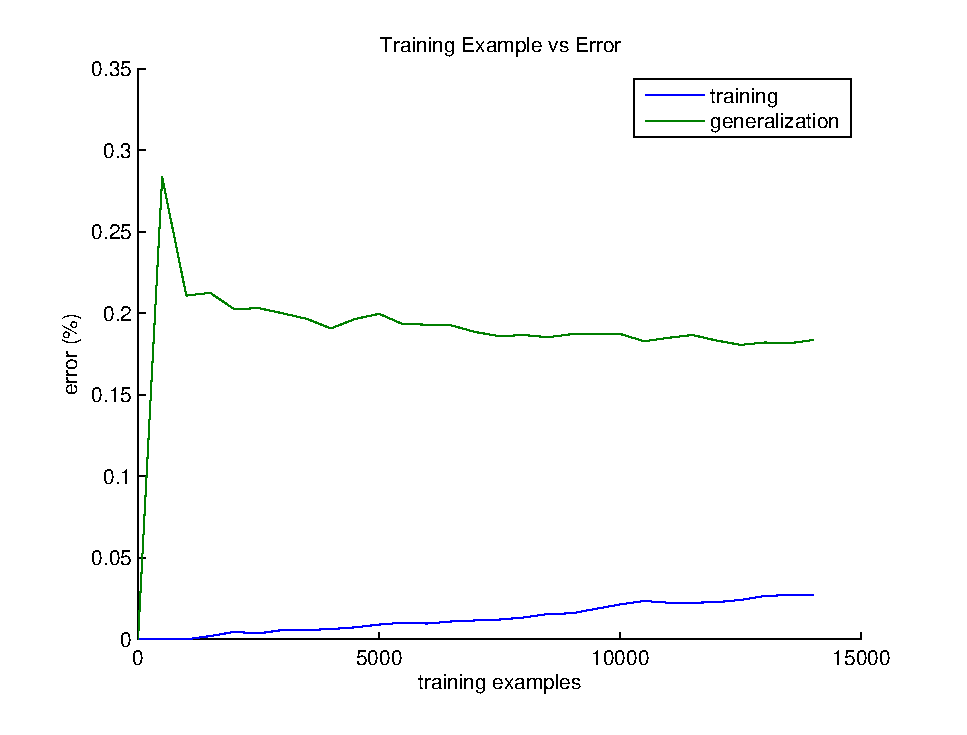
\includegraphics[scale=0.5]{logit-spell-bigram-error}
\par\end{center}


\subsection*{Discussion}

Individually, every data processing technique improved the generalization
accuracy but all of them with the exception of bi-grams, also reduced
training accuracy. When combined incrementally, however, it appears
that stemming and stopword removal actually reduces generalization
accuracy.

From the individual and incremental experiment results, we gathered
that the most promising data processing techniques are spell correction
and bi-grams. Thus we combined only those two and indeed we achieved
training and generalization accuracies that were superior to the rest.

Looking at the training error vs generalization error, it is as expected
that by adding more training examples, the training error (bias) goes
up where as the generalization error (variance) goes down. However
the trend suggests that as we add more training examples, training
error will continue to go up where as the generalization error will
likely flat off. Judging from this we will have to either explore
other pre-processing techniques, other learning algorithms, or other
tuning techniques.



\section*{Further enhancements}

\input{third_attempt.tex}

\input{references.tex}
\end{document}
